\section{Introduction}
\label{sec:intro}

Crowdsourcing provides an inexpensive and efficient method to annotate data for various machine learning tasks 
by employing massive workforce from global Internet users.  
Popular online crowdsourcing service operators include 
Amazon Mechanical Turk\footnote{\url{https://www.mturk.com/}} and CrowdFlower\footnote{\url{http://www.crowdflower.com/}}.  
However, in contrast to expert annotated data, 
crowdsourced annotation usually suffers from relatively higher level of bias.  
Erroneous annotated data might lead to vulnerable performance of trained classifiers 
or imprecise evaluation of tested models, 
which limits the adoption of crowdsourcing as a regular method of annotated data collection.  

Data annotation bias has been studiend in multiple settings.  
Modeling workers' annotating bias on single data items has been studied in a number of studies~\cite{raykar:nips2011ranking,raykar:icml2009,raykar:jmlr2010,whitehill:nips2009}.  
In this scenario, data items are presented separately to the workers 
and no assumption is made on the interference between judgments on different data items.  
We refer to this setting as the \emph{independent judgments}.  
Recently, data items annotated in sequence also attracted research attention~\cite{mozer:nips2010,scholer:sigir2013,scholer:sigir2011}.  
Observing that a worker usually makes judgments on a sequence of data items, 
to some extent there could be dependencies between judgments made on consecutively presented data items.  
This setting could be referred to as \emph{sequential judgments}.  

In this paper, we study another interesting scenario when data items are organized into (small) a batch 
and presented to a worker to be judged together.  
We refer to this setting as \emph{batch judgments}.  
We present a graphical model example of these three different scenarios, as shown in Figure~\ref{fig:worker_mode}.  
Circles represent random variables $y_i'$, which models the annotation given by workers on the $i$-th data item, 
while black boxes represent certain kinds of dependencies.  
Figure~\ref{subfig:mode_ind} shows the scenario when workers make judgments on each data item independently.  
This usually applies when data items are presented to workers separately, 
or when there are rarely correlations between data items.  
Figure~\ref{subfig:mode_seq} as an example of sequential judgments, 
illustrates that there might be dependencies between judgments made on two consecutive data items.  
This case often happens when data items are presented to workers in a sequence, 
and there are some certain correlations between consecutive data items.  
For example, judging the relevance of a list of documents to a fixed query.  
Figure~\ref{subfig:mode_batch} shows the scenario we study in this paper, 
namely when judgments are made simultaneously to a batch of data items.  
This scenario usually happens when workers are required to make judgments to several data items at the same time, 
or the data items in the same batch are strongly connected.  
Notice that the size of batch is usually relatively small (\eg~$\leq 5$) 
because a worker usually cannot pay attention to more data items at the same time.  
When the batch becomes too large, the scenario might be reduced to the case when workers make sequential judgments.  



This judging-in-batch setting has been noticed and adopted in crowdsourcing practices of 
object recognition~\cite{su:aaai2012}, clustering~\cite{gomes:nips2011}, and sorting~\cite{marcus:vldb2011}, 
which facilitates some tasks requiring workers to judge data items based on comparison, 
also benefits other tasks on efficiency and cost.  
However, little research has explicitly addressed this setting and studied the annotation bias.  
Our previous research~\cite{zhuang:wsdm2015} also noticed this specific type of annotation bias, 
but instead of focusing on debiasing, 
we exploited the bias to develop an active learning algorithm aiming to improve a certain classifier performance.  



\begin{figure}[!t]
  \centering
  \subfigure[Independent judgments]{
    \label{subfig:mode_ind}
    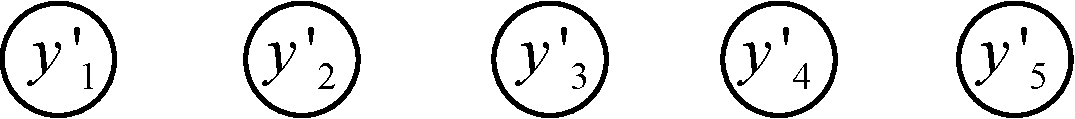
\includegraphics[width=0.95\columnwidth]{figures/mode_ind}
  }\\
  \vspace{0.2in}
  \subfigure[Sequential judgments]{
    \label{subfig:mode_seq}
    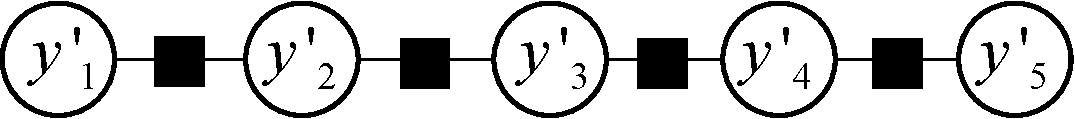
\includegraphics[width=0.95\columnwidth]{figures/mode_seq}
  }\\
  \vspace{0.2in}
  \subfigure[Batch judgments]{
    \label{subfig:mode_batch}
    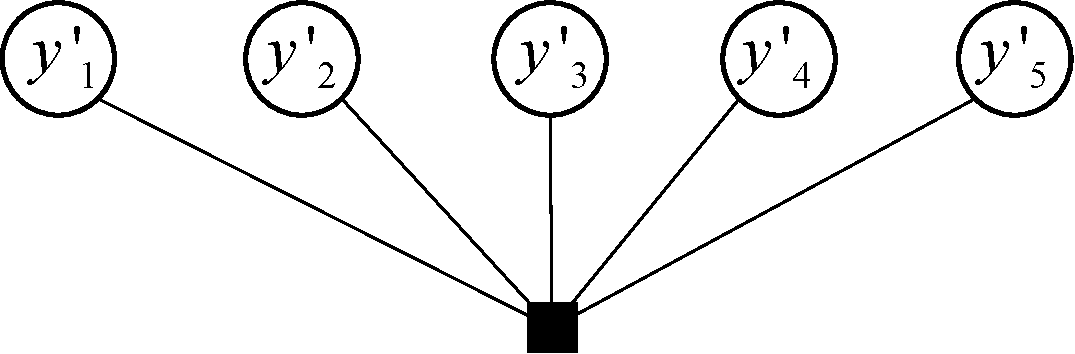
\includegraphics[width=0.95\columnwidth]{figures/mode_batch}
  }
  \caption{\label{fig:worker_mode}
  Graphical model examples of three different scenarios of crowdsourced annotation: 
  independent judgments usually occur with interfaces where data items presented separately; 
  sequential judgments apply to the case when data items are presented in a long sequence;
  batch judgments usually apply to the scenario when data items are presented in a relatively small batch.  
  Circles of $y_i'$ denote random variables representing the annotation given by workers, 
  while black boxes are factor functions modeling the dependencies.  
  }
\end{figure}

There are several research challenges in studying this problem.  
First, how to model workers' behavior when they make judgments in batches?  
Second, how to leverage the model to debias the crowdsourced annotation of data batches?
The following contributions are made regarding these questions:
\begin{enumerate}
  \item \emph{Proposing an interpretable worker annotation model on small batches of data.}
        We propose a novel worker model for binary annotating behavior with data items organized in small batches.  
        The model incorporates independent judgments and batch judgments based on ranking.  
        Different from the factor graph model in our previous work~\cite{zhuang:wsdm2015}, 
        our novel model is more interpretable.  
  \item \emph{Debiasing annotation data obtained as batches.}
        Based on our proposed worker model, we provide an algorithm to debias the inferred labels 
        when they are collected from data items in small batches.  
  \item \emph{Conducting experiments on real-world crowdsourcing platform.}  
        We conduct experiments on both synthetic and real-world crowdsourcing data sets 
        to verify the effectiveness of our proposed model and debiasing strategies.  
        Experimental results show the effectiveness of our debiasing method over other baselines.   
        %the F1-score of the inferred labels on the real data set can be raised from 88\% to 90\%.  
\end{enumerate}

The rest of this paper is organized as follows:
Section~\ref{sec:prelim} introduces the background of crowdsourcing, and formalizes the research problem;
Section~\ref{sec:worker} proposes the worker model for annotating small batches of data;
Section~\ref{sec:debias} presents a strategy to debias batch annotations;
Section~\ref{sec:exp} illustrates experimental results;
Section~\ref{sec:related} introduces related work and Section~\ref{sec:conclusion} concludes. 






